\documentclass[11pt,journal]{IEEEtran}

\usepackage{times}
\usepackage{amssymb}
\usepackage{amsmath,amsfonts}
\usepackage{amsthm}
\usepackage{graphicx}

\usepackage{color}
\usepackage{xcolor}

\usepackage{scalefnt}

\usepackage{pgf}
\usepackage{tikz}
\usetikzlibrary{shapes.symbols,shapes.callouts,decorations,shapes.geometric,arrows}

\usepackage{hhline}
\usepackage{multirow}
\usepackage{array}
\usepackage{pdfpages}
\usepackage{subfigure}
\usepackage{algorithm}
\usepackage[noend]{algpseudocode}
\usepackage{balance}
\usepackage{epsfig}


\newcommand{\todo}[1]{} %essentially a block comment

\newtheorem{theorem}{Theorem}
\newtheorem{definition}{Definition}
\newtheorem{lemma}{Lemma}

\hyphenation{designs design algo-rithms devel-oped micro-pipeline after
  algo-rithm AFSM AFSMs}

\begin{document}

\title{Smart Chess Board}

\author{Nicole Sundberg, Griffin Rodgers, Kenan Ntambwe, Jack Marshall
  \thanks{The authors are in the Computer Engineering
    department at the University of Utah.}
}
\maketitle


\begin{abstract}
Chess is an incredibly fun game, but can often feel extremely intimidating to newcomers. With a variety of specialized pieces that each have their own movement scheme, learning and having fun with chess can feel like a lofty goal for those that have never played before. Furthermore, increasing your skill and understanding of chess can be difficult when games become complicated and difficult to recall. For these reasons, the Smart Chess Board was created.  The Smart Chess Board is a chess board that teaches players how to play chess by clearly indicating possible moves when pieces are lifted.  The board also records moves alongside an application that tracks game statistics and more so that even seasoned chess players can retrospectively analyze their gameplay. The board will indicate possible moves via LEDs under the chess squares and will keep track of pieces lifted or moved. An application will also display the results and progress of the match per account. An AI algorithm will allow the player to play on the chess board against a computer player so that learning can happen even without a chess partner. 
\end{abstract}

\section{Introduction}

\IEEEPARstart{C}{hess} is a world-known and widely enjoyed game. However, its complexity leaves many potential players struggling due to the many pieces, rules, and movement schemes. In an effort to create a fun and easy way to teach new chess players along with supplement the learning of more experienced players, the Smart Chess Board was created. 

This chess board allows new and experienced chess players to benefit by showing possible moves and checking rules but also recording match history for virtual playback through the companion application. The Smart Chess Board shows players legal moves by lighting up the squares when pieces are lifted. The board also detects invalid or illegal moves and alerts the players with the board lights as well.  The chess board will work alongside the companion application to record times and game history, allowing for clear growth and progress to be shown to players as they look through their previous games. The board also allows single-player mode where users can learn without the need of another physical chess player, allowing for easy learning at any time or place.

Using sensors and bluetooth connectivity, the board is able to determine when pieces are picked up or put down and record game data. Through algorithmic checking and the use of LED lights the board will also determine move legality and visualize legal moves when a piece is picked up.

%** \textbf{TODO: describe comparisons to other solutions, advantages to this one} **
There are programs designed to teach newcomers chess, but they do not often pair with a physical board. The creation of a physical board allows for more tactile learning styles and for users to learn in a more hands-on way that promotes a better understanding of the game overall. On top of this, these programs often do not allow for virtual replaying matches to determine mistakes or errors made or saving and tallying game statistics to show overall progress. Because of this, the Smart Chess Board is a more active and well rounded solution that is better able to engage the audience.


% Refer to figures as follows:
% The circuit in Fig.~\ref{fig:circuit}.

% Citations are as follows
% Algorithm returning longest netlist delay path \cite{knuth:book1973}.
%\subsection{Project Demonstration}
To demonstrate the Smart Chess Board, the physical custom chess board along with the running companion app will be available to interested parties. When they lift a piece on the board, all valid moves and their associated squares will light up on the board, and once the piece is placed on a valid square, that move is logged by our app that is connected to the board. The player would also have the option of playing against a chess AI, and the opposite end of the board will indicate which pieces needed to be moved on behalf of the AI when the AI takes its move. The application will also have a co-demonstration where we can showcase the game history functionality and allow the user to play back previously played games.

\section{Background}



\subsection{Related Work}

Similar products to our chess board design are on the market as both commercial products and open-source hobbyist projects. These products generally suffer from at least one of the following problems: high cost, requires access to specialized tools (e.g. 3D Printer), or lack quality of life features. Despite these shortcomings, many of them contain other novel features, such as move assistance, where you can enable and configure the board to suggest optimal moves in the current game, or multi-colored LED indicators to indicate the strength of a move. We have found two examples of smart chess boards, one from the consumer space and the other from academia, and will provide a short explanation of their functionality as well as our criticisms with each design.

% You may want to subsection the background.

% Include plenty of figures.

%% This is a figure with two side by side images.
% \begin{figure}[thb]\centering
%   \begin{minipage}{0.48\columnwidth}
%     \centerline{\psfig{file=images/IMG_2712-crop.jpg, height=30mm, angle=0}}
%     \begin{center} (a) \end{center}
%   \end{minipage}
%   \begin{minipage}{0.5\columnwidth}
%     \centerline{\psfig{file=images/img2.png, height=30mm, angle=0}}
%     \begin{center} (b) \end{center}
%   \end{minipage}
%   \caption{The die and substrate (a), and complete system (b).}
%   \label{fig:chip-system}
% \end{figure}

% This is how you label a section of the text:
% \label{sec:falsePath}
ChessUp is a smart chess board that was funded via Kickstarter. Some of its features include LEDs to signal correct/incorrect moves, a companion app allowing play against friends and family, and unique ''touchsense pieces'' that can detect when a piece is touched and show the available moves for that piece \cite{chessup}. In our research of the ChessUp, we noticed that to access some basic features, such as the chess clock, requires a smart phone with the ChessUp app installed and placed next to the board and left there for the entire game. We also noticed reviews stating that the app connectivity is finicky, with apparent disconnects from online games as well as no indication of when the opposing online player has resigned from the game, other than ceasing to make moves.

Assistive Chess board is a project proposal from a group of electrical engineering students at the University of Illinois in Fall 2017. This project proposal details an assistive chess board project that is very similar to the one proposed here. However, this proposal only details the hardware implementation of the board, and does not cover any software components at all other than a passing mention of a mobile app that communicates with the board via Bluetooth. The Assistive Chessboard implements features such as entirely wireless play, with the integration of the previously mentioned Bluetooth and a rechargeable battery, enabling a wireless playtime of up to 4 hours. It uses hall-effect sensors under each square of the chess board to detect if a piece is placed on any given square. In addition, it also uses multi-colored LEDs to signal to the player whether a move is correct or incorrect. It also integrates a basic LCD display and various buttons for user interactivity, however the details are scant on how these were to be implemented. One novel feature here is the use of a 24-bit shift register to select and manipulate the color of the integrated LEDs. The authors also designed custom PCBs for each of the squares of the board containing the LED and sensor circuits \cite{assistivechess}. We believe that this is a good approach for prototyping as it allows for fast diagnosis and swapping of PCBs if a fault is detected, however this does make wiring and overall organization of the board more complicated.
% You can include equations such as Eqn.~\ref{eqn:booleanDifference}
% \cite{boole:book1872}.

% \begin{equation}
%   \frac{df}{df_x} = f_x \oplus f_{\overline{x}}
%   \label{eqn:booleanDifference}
% \end{equation}



\section{Proposed Work}

\subsection{Project Synopsis}
The Chess Board will consist of an MCU, a Raspberry Pi Pico WH, that serves as the interface between the software and hardware components. The sensor block(s) consisting of DRV5053 Hall-effect sensor and supporting components will be connected to the MCU via eight external 8 channel ADCs, one for each row of the chessboard. The user-interface buttons will be directly wired to GPIO headers on the MCU. The MCU will output game data to both an LCD Display and the various LEDs integrated in the board via I\textsuperscript{2}C. The Chess Board will communicate with the external smartphone application via Bluetooth connectivity, to send and receive data about the state of the current game. The app will communicate with a selected online chess API (Lichess, chess.com, etc.) as well as a database to archive the current and previous games played on the board. Refer to Fig. \ref{blockdiag} for a simple block diagram representing the chess board.

\begin{figure}[h]
  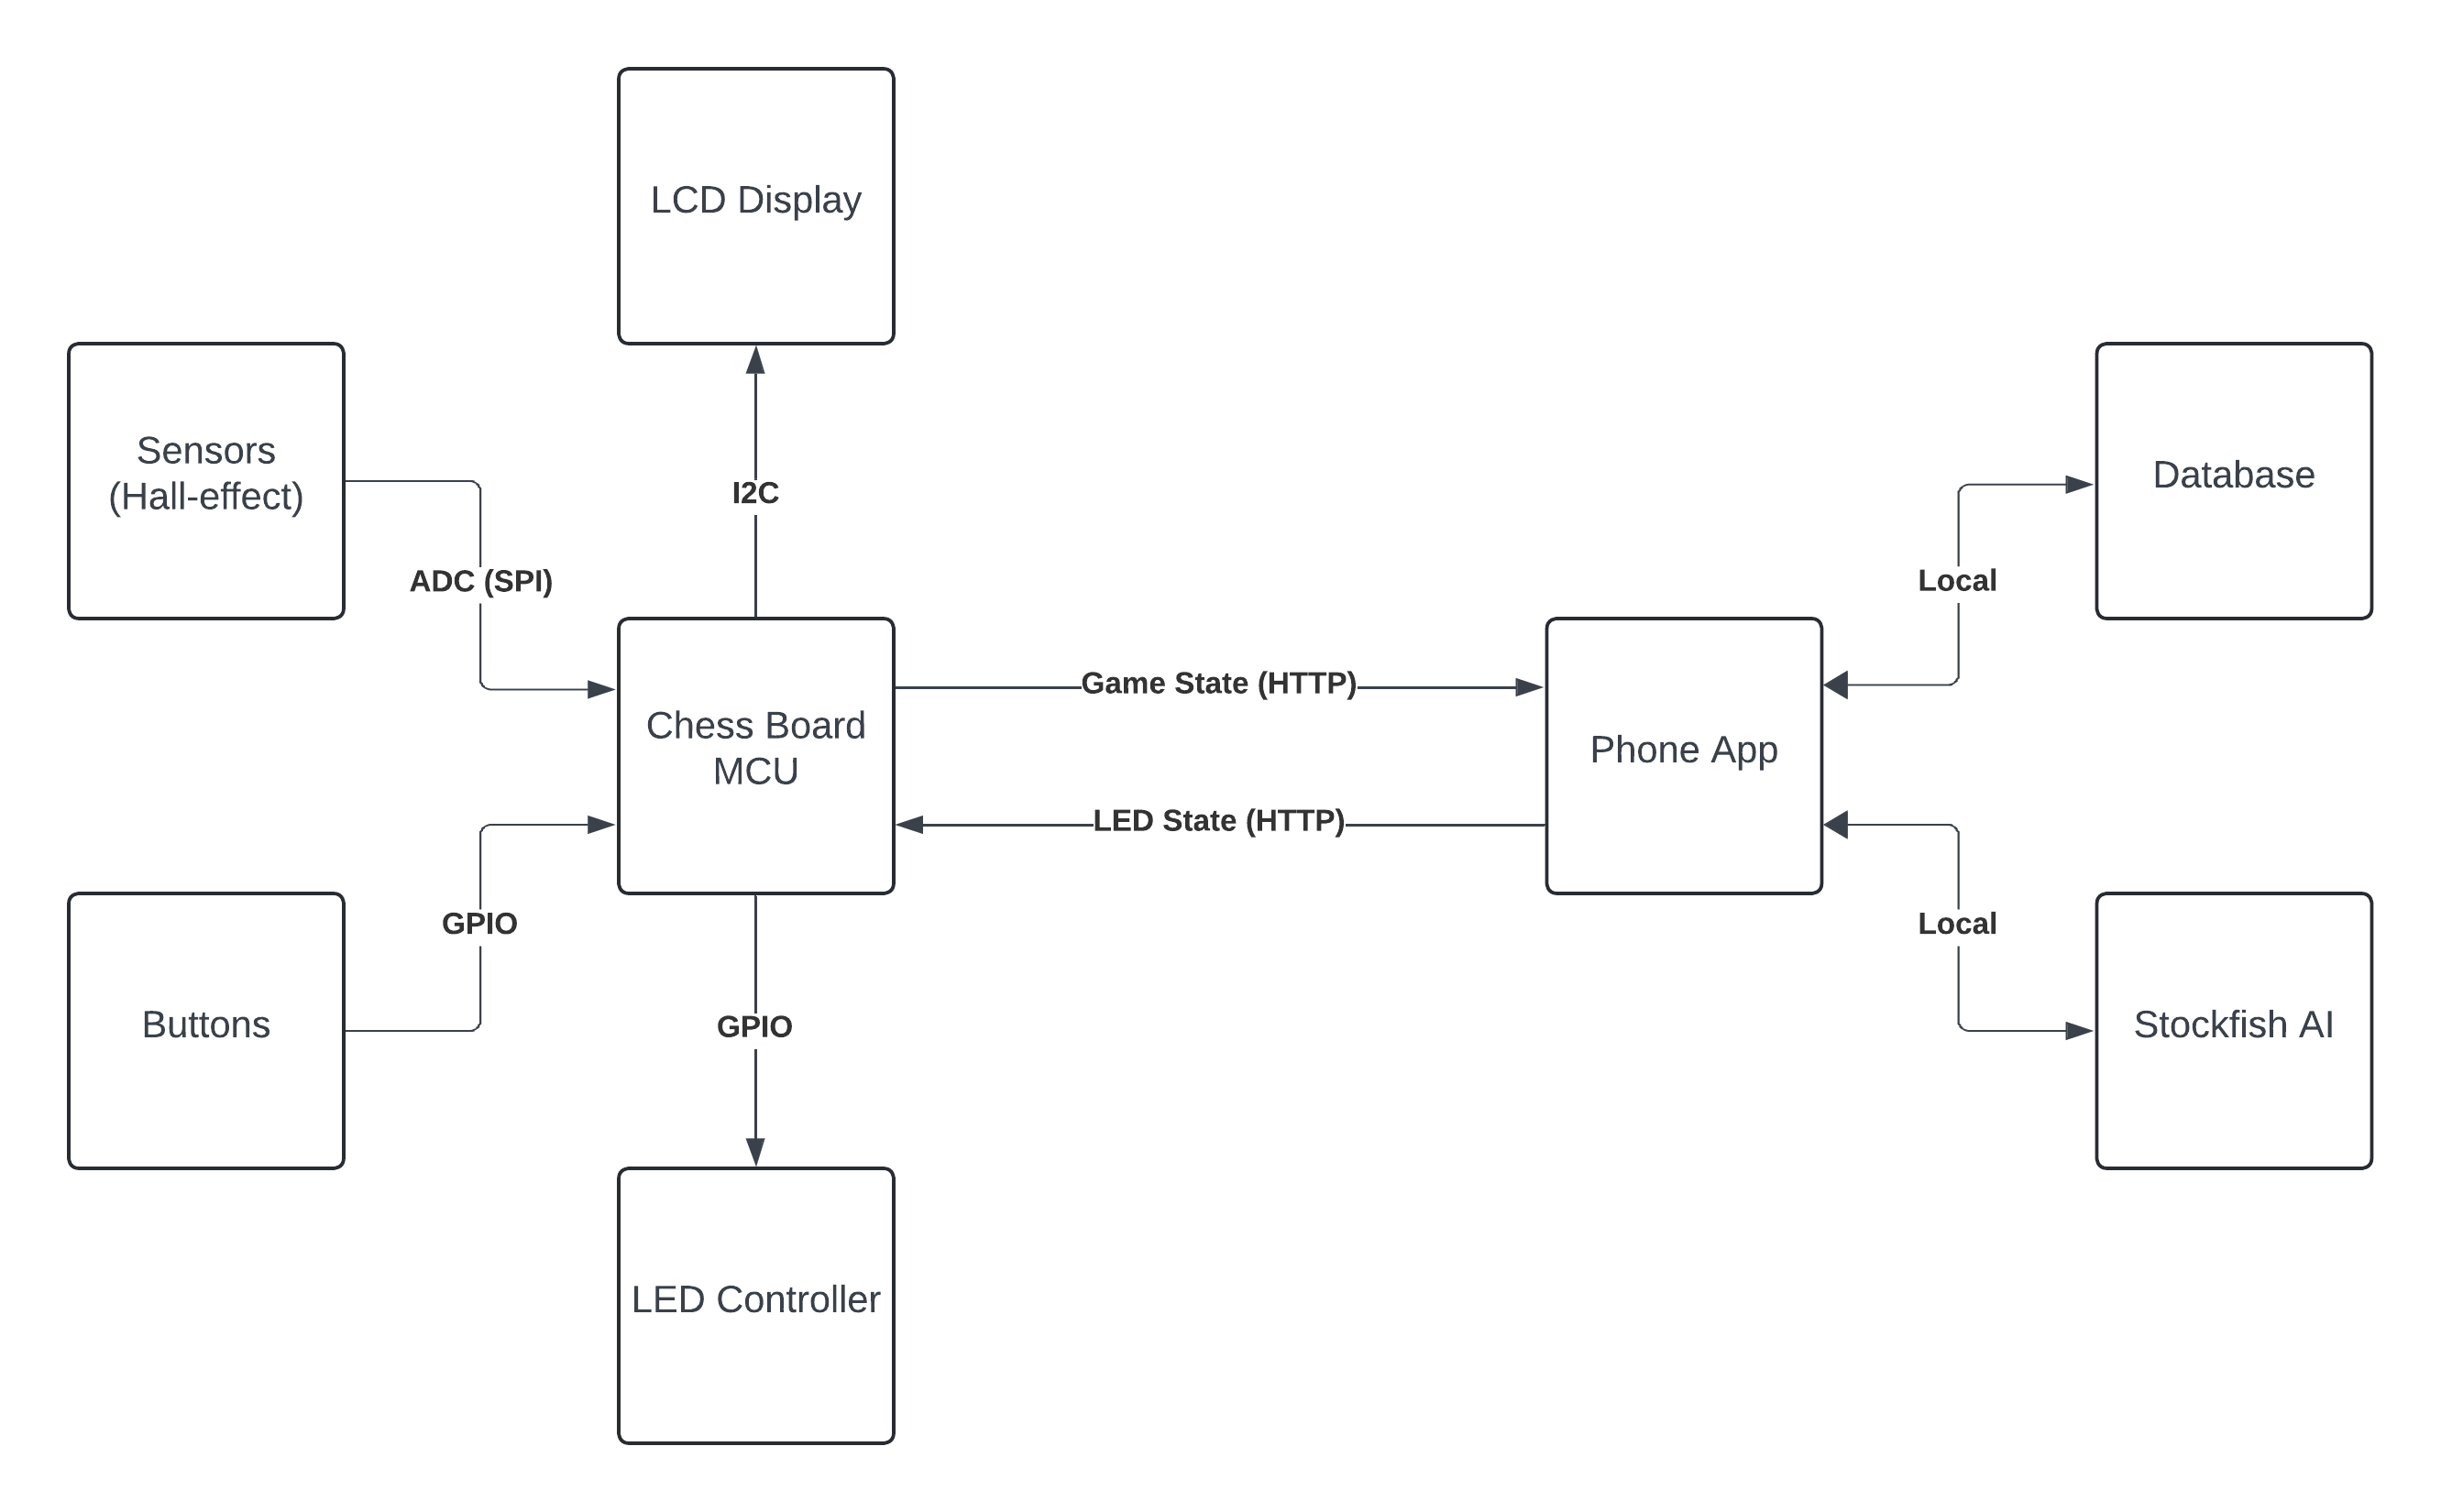
\includegraphics[width=\linewidth]{Chess Board Capstone Block Diagram}
  \caption{Block Diagram}
  \label{blockdiag}
\end{figure}
%%
% This section should start out with a detailed description of the implementation.  
% A block diagram would be very helpful, as it defines the major components and 
% interfaces.  Each interface between components needs to be defined between hardware 
% and hardware and software.  What algorithms are you using?  What components are you 
% using?  Will they be purchased or built from scratch?   etc.
%%


\subsection{Sensors}

For the Smart Chess Board project, special sensors are needed in order to keep track of the pieces on the board. One type of sensor is called an optical sensor, which can see where the pieces are placed. Tiny cameras or sensors can be used that can detect invisible light to do this. Another type is a pressure sensor, which can feel when a piece is put on or taken off the board. These sensors are like tiny detectors under each square on the board. Motion sensors can be used to sense when the board is moved or tilted. These sensors can make it easier for players to control the game without touching anything. Finally, sensors that detect magnetic fields could be used alongside magnetic chess pieces to determine when pieces are moved. Using these sensors, the Smart Chess Board cane be made to be fun and accessible to everyone.




\subsection{Team Responsibilities and Milestones}
The Smart Chess Board project consists of the following parts: board hardware, board-to-application communications, application design, and application programming interface or API alongside database management. All portions will be responsible for their own testing and documentation in order to ensure each individual portion works as expected and can be easily understood. Overall, Jack will work on the communications portion, Kenan will work on the board hardware, Griffin will work on the API and database management, and Nicole will work on the application design.

The following is our milestone schedule:


\textbf{Basic Functionality (through June 5th 2024):} Create a single testing square for the board. Allow this square to determine if a piece is placed/picked up and show it visually. Begin application design, have very basic downloadable prototype. Plan and document database and API usage as well as hardware-software communications.

\textbf{Minor Integration (through September 2024):} Have multiple squares for the board. The squares should now have communications implemented to the app. The application should show changes in the squares visually. Saving moves to the database should now be implemented.

\textbf{Final Integration (through December 2024):} All board pieces should be completed and polished. All communications between the board and the application should be implemented. The application should allow for replaying previous games virtually. API to chess.com or other sources should work to allow for AI games to be played. 



\subsection{Team Management}

A team discord and group chat has been created to maintain easy communication between team members as well as easy resource storage as the project work and designs are completed. A github project and associated task board has also been created to ensure work on tasks proceeds as expected and all team members can see work as it progresses. Notetaking as well as progress updates have been left to Nicole to minimize any issues with switching team members and schedules per week.

\subsection{Testing And Integration}
To ensure smooth integration and final products, incremental testing and integration will occur throughout progress on the Smart Chess Board. As per the previously described milestones, integration will go through several phases: basic functionality in which designs are planned but integration has not yet begun, minor integration in which the physical board begins to communicate with the application and database work is set up, and final integration in which all connections are built and finalized in accordance with project designs.

In order to maintain stability across all sections of the project, integration plans for databases, communications, and API connectivity will be planned and determined prior to integration steps. Incremental and unit testing will occur on each component of the project (board-to-application communications, application design, and API/database management) prior to their integration. This way, each individual piece is guaranteed to work as specified before complicating the project with connected pieces working together.

A protocol for data transference between the board and application will be determined and tested via fake transfers and dummy data to ensure stability. Unit testing will occur on the app to ensure data structures are properly built and user interface is stable. Manual testing will be done for the board to ensure each component works properly and sends the appropriate data to the Raspberry Pi.

\subsection{Risk Assessment}
Some concerns for this project include the possibility of magnets interfering with the planned circuitry. This is a medium risk, as it isn't completely likely to occur and there are measures to be taken to minimize this problem impacting the project. To ensure that the project may continue through these issues, the plan is to build several prototypes for the squares before creating the final board. These prototypes will include different sensors and setups to ensure that a solution is found that will best work for the whole board. After prototyping these different squares, the best option will be determined in terms of which design to follow for the rest of the board.

It is also possible that issues might present themselves with connecting to the Chess.com APIs. Since these APIs are controlled by outside sources and usability might change, guaranteeing that the APIs will work as expected is impossible. Since this is an API that is used in other projects and is relied on by other services, the likelihood of these issues is very low, making this a low risk concern. In the case that the APIs are unable to be used in the planned manner, there are several possible solutions. The first is to create a simple minimax algorithm to determine a decent and valid move. The second solution would be to use another API, since there are other solutions available. The third is to use an existing chess AI project available on the internet and integrate it into our existing project while giving credit to the original creators. In any case, there are several options to guarantee the functionality even without the API working as expected.

There is also a high probability of setbacks and issues with integrating all of the sections of the project. Because they will be developed independently, there is always risk of the individual aspects not integrating easily. However, this is a medium or low risk concern since our milestones and testing/integration plans are based on an incremental integration process that will allow problems with integration to be found early and be solved before the project sections get overwhelmingly complicated. Once the minor integration milestone is complete, this will minimize to a low risk concern.


\subsection{Bill Of Materials}
The Smart Chess Board needs a physical, custom made body in addition to several hardware components. The following lists the materials used. The components will be listed in the order of quantity, part description, vendor, and unit price. Refer to Table \ref{bomtable}.
\begin{center}
\begin{table}[ht]
\caption{Bill of Materials}
\begin{tabular}{|l|l|l|l|}
\hline
\textbf{Qty} & \textbf{Part}                        & \textbf{Source} & \textbf{Price}          \\ \hline
1            & Roll of LEDs                         & Amazon          &                         \\ \hline
64           & DRV5053 Hall-effect  sensor          & DigiKey         &                         \\ \hline
1            & 1kg PLA Filament                     & Amazon          &                         \\ \hline
1            & Raspberry Pi Pico WH                 & PiShop.us       &                         \\ \hline
32           & N42 Neodymium Magnet 1.26"           & Amazon          &                         \\ \hline
8            & Adafruit ADS7830 ADC                 & Adafruit        &                         \\ \hline
1            & USB Power Delivery board             & Amazon          &                         \\ \hline
\end{tabular}
\label{bomtable}
\end{table}
\end{center}
% You probably want subsections for tasks, testing and integration,
% management and communication, schedule and milestones, risk
% assessment, bill of materials (not necessarily in this order)


% \section{Results}
% \label{sec:results}
% 
% This section probably won't be in the proposal.


\section{Conclusion}



\section*{Acknowledgment}

Include this section if needed.

The authors would like to thank \ldots



\bibliographystyle{IEEEtran}  % IEEEtran -- needs IEEEtran.bst
% Balance the citations to equalize the columns manually
% \balance
\bibliography{proposal}

\end{document}


% LocalWords:  Eqn df
